\chapter{Funkčnosť, výsledky testovania}

\indent\indent OMNeT++ ponúka veľmi efektívne nástroje na spracovávanie výsledkov simulácii. Jedným z nich je aj tzv. Event Log Viewer. Priebeh simulácie vrátane popisu zasielaných správ, stavov a ich väzba na simulačný čas sú zaznamenávané do súboru. Následne je možnosť tieto priebehy spracovať cez zásuvný modul v nástroji Eclipse, ktorý je dodávaný spolu so štvrtou hlavnou verziou simulátora. Takýmto spôsobom sú na nasledujúcich stranách tejto kapitoly vyobrazené a popásanie niektoré zo základných implementovaných sekvencii z nášho modelu.\\
\indent Na prvom z uvedenej série~\ref{fig:chart_init} je sekvencia opisujúca úvodnú postupnosť správ pre vytvorenie siete PAN koordinátorom. Na sieťovú vrstvu entitou \texttt{NLME} je prijatá správa NLME-NETWORK-FORMATION.request, ktorej obsah definuje konfiguračné parametre siete, ktorú chceme vytvoriť. Podľa akceptovanej množiny kanálov sú spustené procedúry pre preskenovanie kanálov a zistenie ich energetických hladín. Pre každý kanál to predstavuje vykonanie série testov, z ktorých \texttt{MLME} vrstva si vyberie ten pesimistický variant. Po vykonaní analýz na sa spustí tzv. aktívny sken na požadovaných kanáloch. Ten je doprevádzaný vysielaním požiadavku pre zaslanie beacon rámca. Po spracovaní výsledkov sa zapíšu konfiguračné premenné do informačnej bázy \texttt{NWK-PIB} a \texttt{MAC-PIB} a začína sa s rozposielaním beacon rámcov~\ref{fig:chart_beacon} (v prípade, že sa jedná o beaconing mód). Na príslušnom obrázku je vidieť, že simulátor pracuje aj rýchlosťou šírenia signálu. To je ošetrené modulom \texttt{ChannelControl}. V prípade zvolenia vhodného kandidáta ako rodiča pre začlenenie sa do siete sa môže vyslať požiadavka pre asociáciu do siete. Táto správa je poslaná v CAP perióde. Na príslušnom grafe~\ref{fig:chart_associate_request} je možné spozorovať časovač CAP slot timer, ktorý určuje začiatok a koniec CAP slotov. Associate Request Command požiadavok je posielaný (tak isto, ako iné riadiace správy) vždy na začiatku nového CAP slotu. Ďalej je daný obrázok zobrazuje posielanie potvrdzujúceho rámca (žiadosť o asociáciu vyžaduje potvrdzovanie), ktorý je iniciovaný v \texttt{MCPS} vrstve cieľového zariadenia. Po uplynutí periódy o dĺžke \textit{macResponseWaitTime} symbolov môžme na sekvencii znázornenej na obr.~\ref{fig:chart_data_request} pozorovať transfer rámca typu Data Request Command z vrsvty \texttt{MLME} do vrstvy \texttt{MCSP}, ale aj keď už je obsiahnutý v tejto fronte, čaká sa na začiatok nového CAP slotu (časovač CAP slot timer), ktorým sa vyšle \texttt{PLME} vrstve príkaz na vykonanie CCA procedúry. V prípade, že tá detekuje kanál v stave \textit{IDLE}, je Data Request Command príkaz poslaný cieľu. Prijatie takéhoto rámca je tiež potvrdené ACK rámcom. Odpoveďou potom bude vyslanie Associate Response Command príkazu (obr.~\ref{fig:chart_associate_response}).\\
\indent Z dôvodu zjednodušenia modelu je možné v jeden okamih asociovať len jeden uzol. Každý ďalší požiadavok o asociáciu bude ignorovaný.\\

\begin{figure}[htbp]
\begin{center}
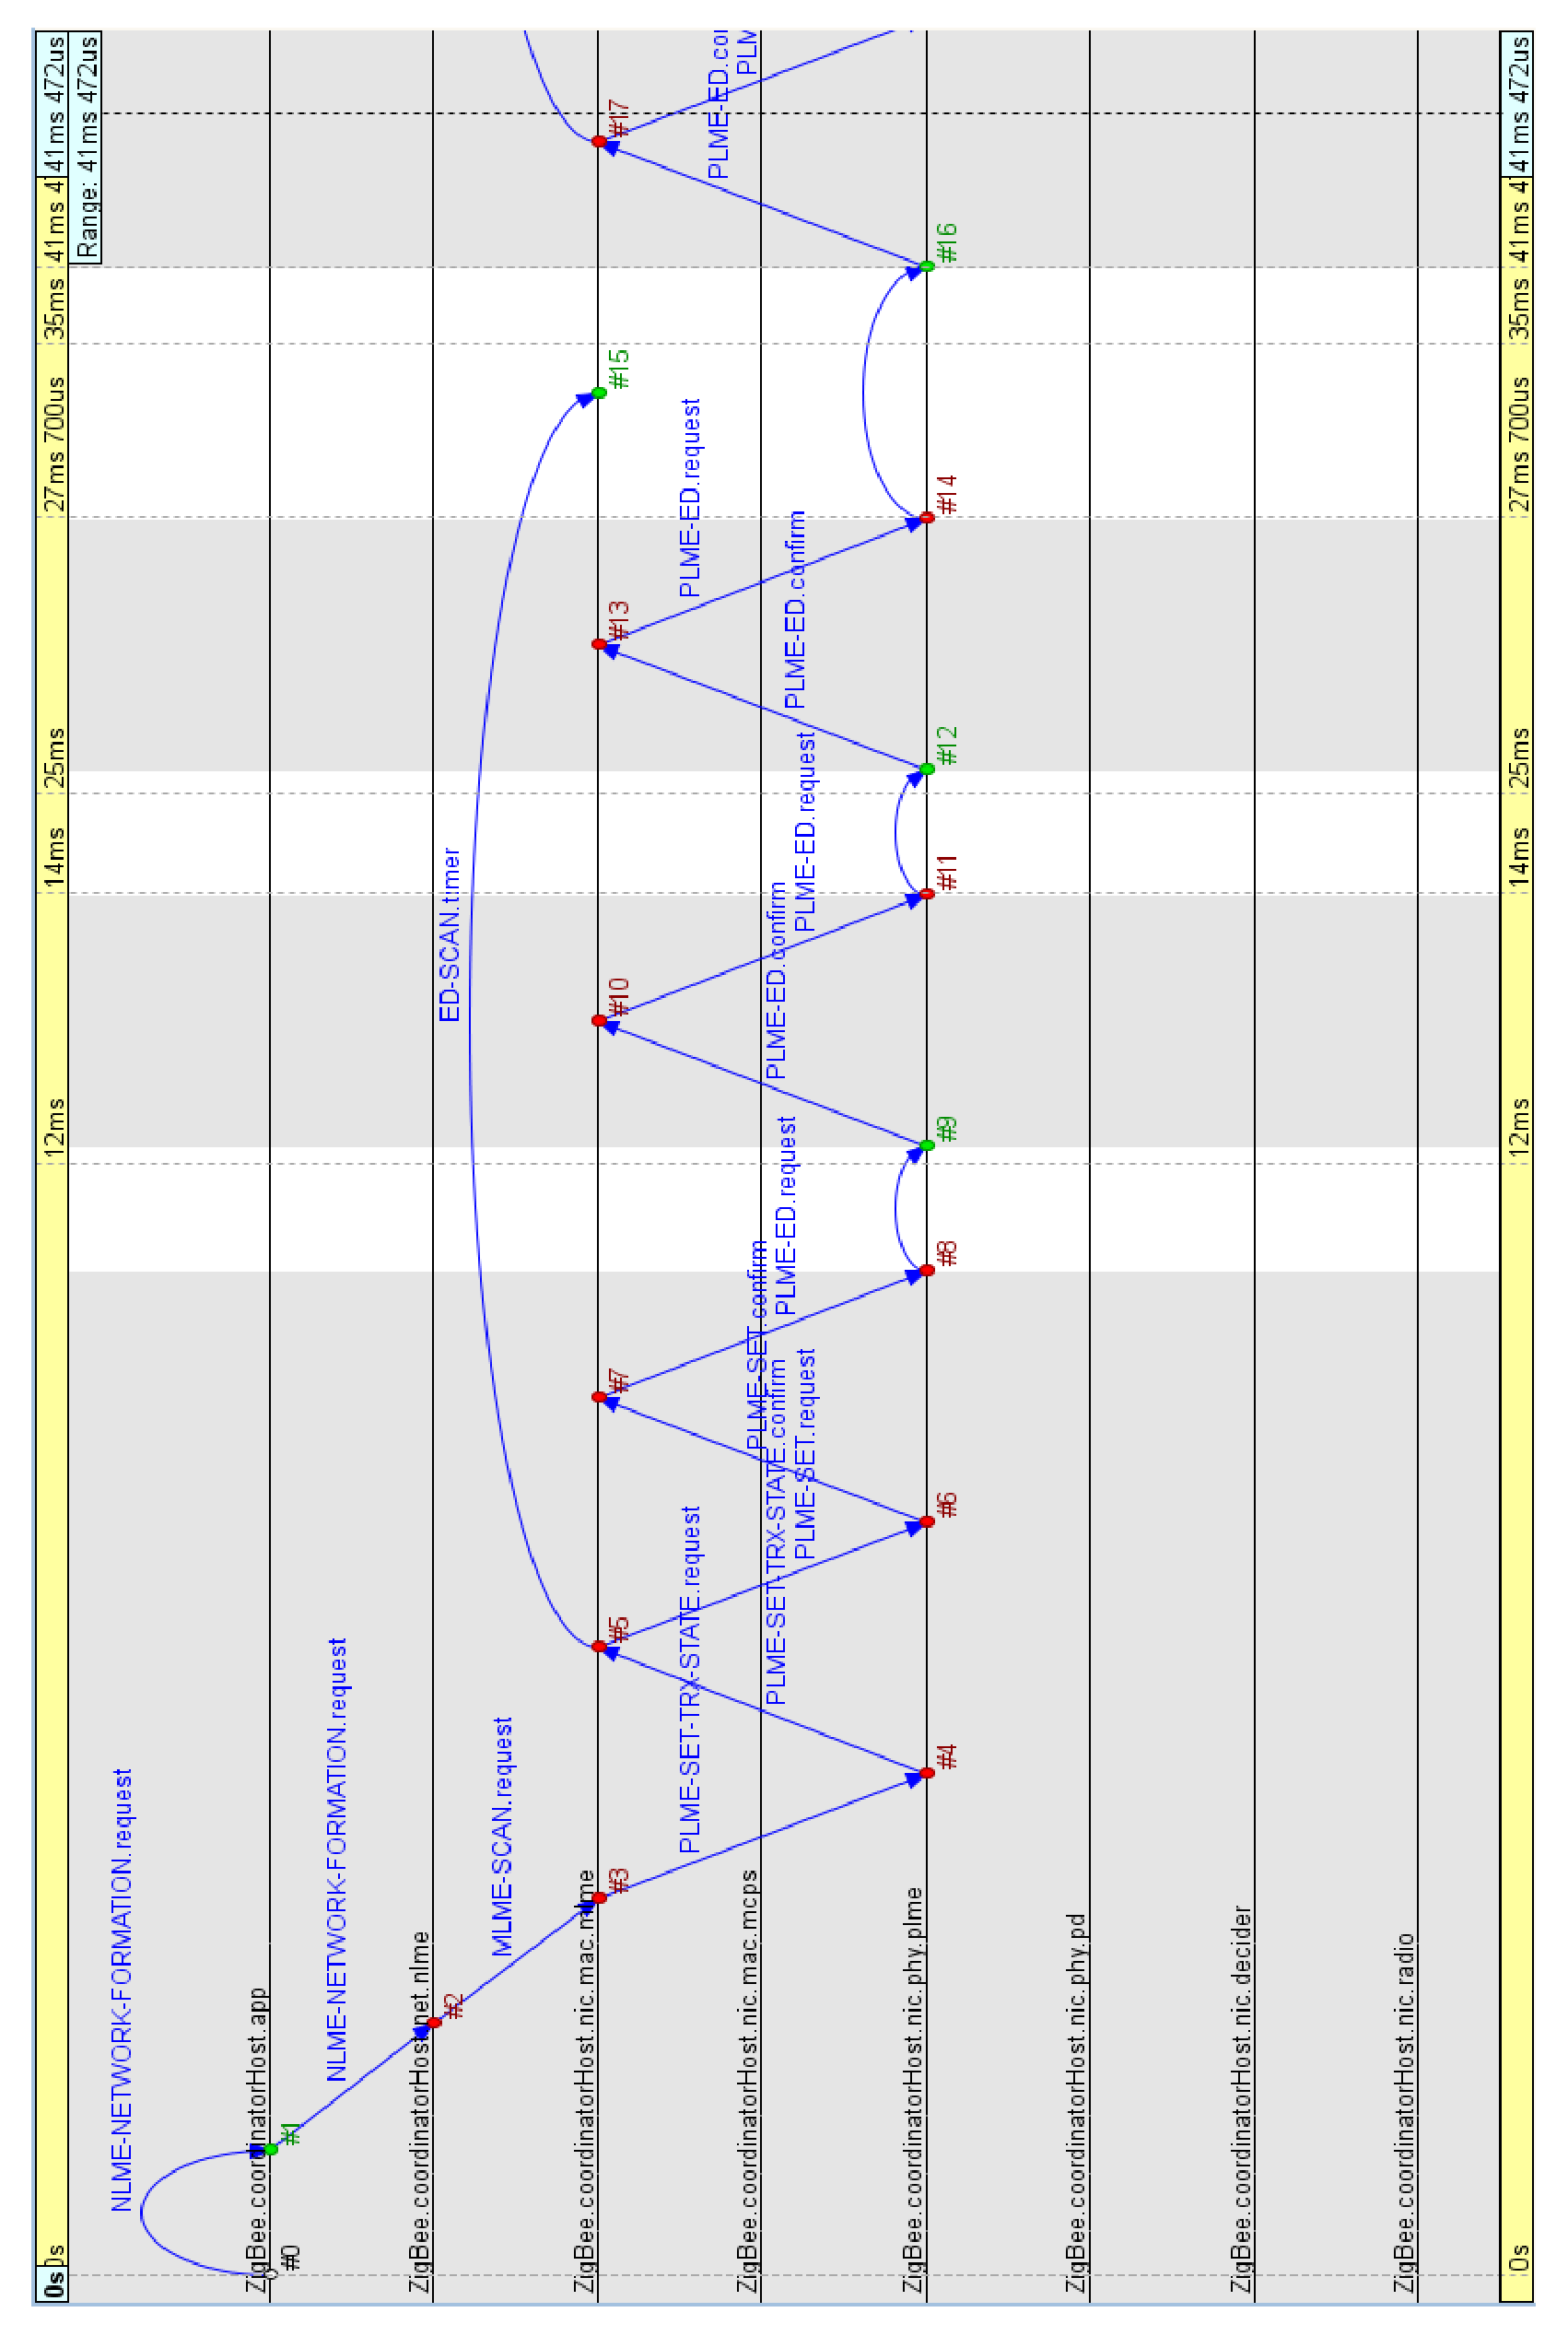
\includegraphics[width=140mm]{figures/chart_init}
\caption{Inicializácia koordinátora, ED sken}
\label{fig:chart_init}
\end{center}
\end{figure}

\begin{figure}[htbp]
\begin{center}
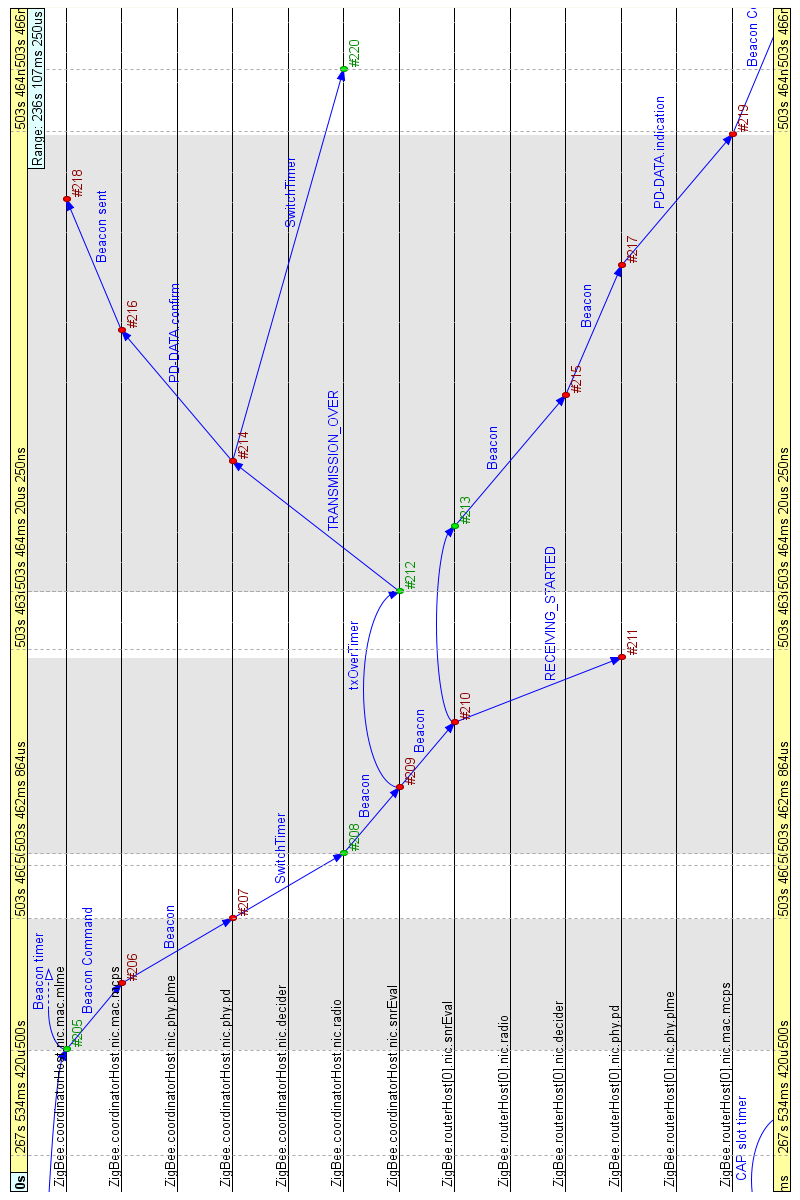
\includegraphics[width=140mm]{figures/chart_beacon}
\caption{Vysielanie a prijatie beacon rámcov}
\label{fig:chart_beacon}
\end{center}
\end{figure}

\begin{figure}[htbp]
\begin{center}
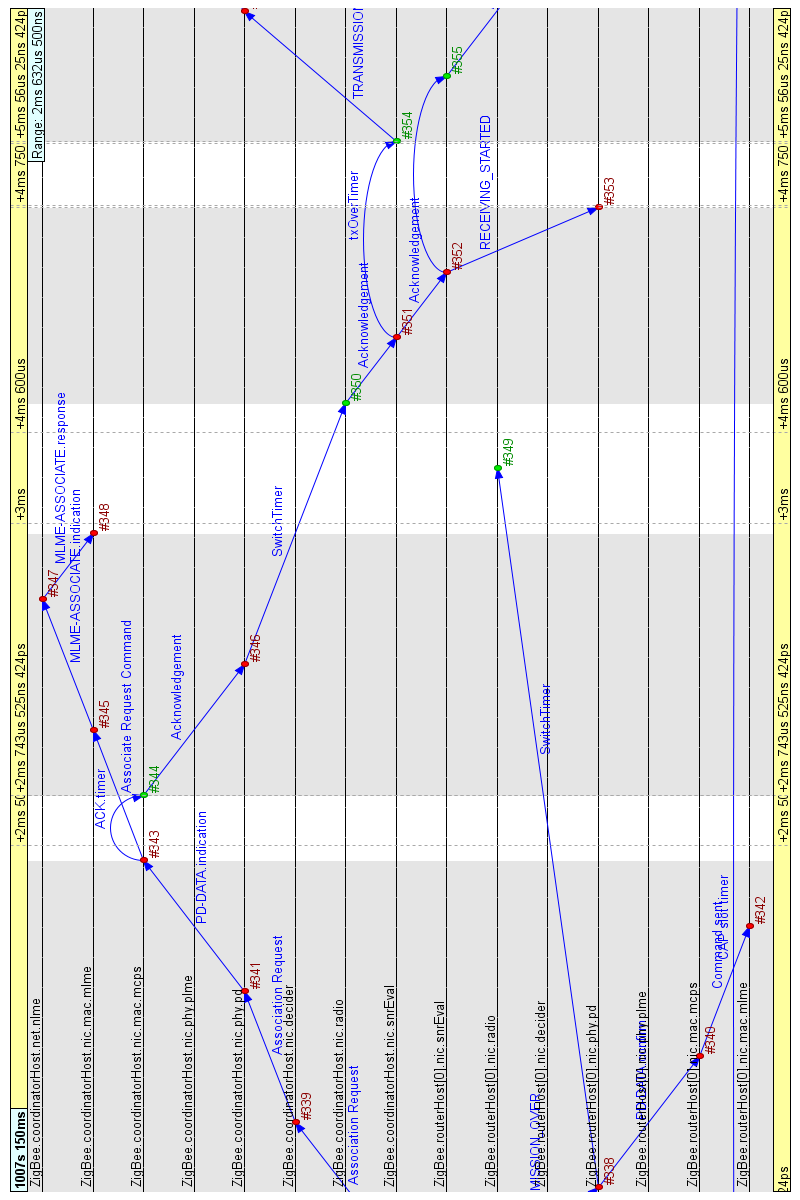
\includegraphics[width=140mm]{figures/chart_associate_request}
\caption{Spracovanie žiadosti o asociáciu}
\label{fig:chart_associate_request}
\end{center}
\end{figure}

\begin{figure}[htbp]
\begin{center}
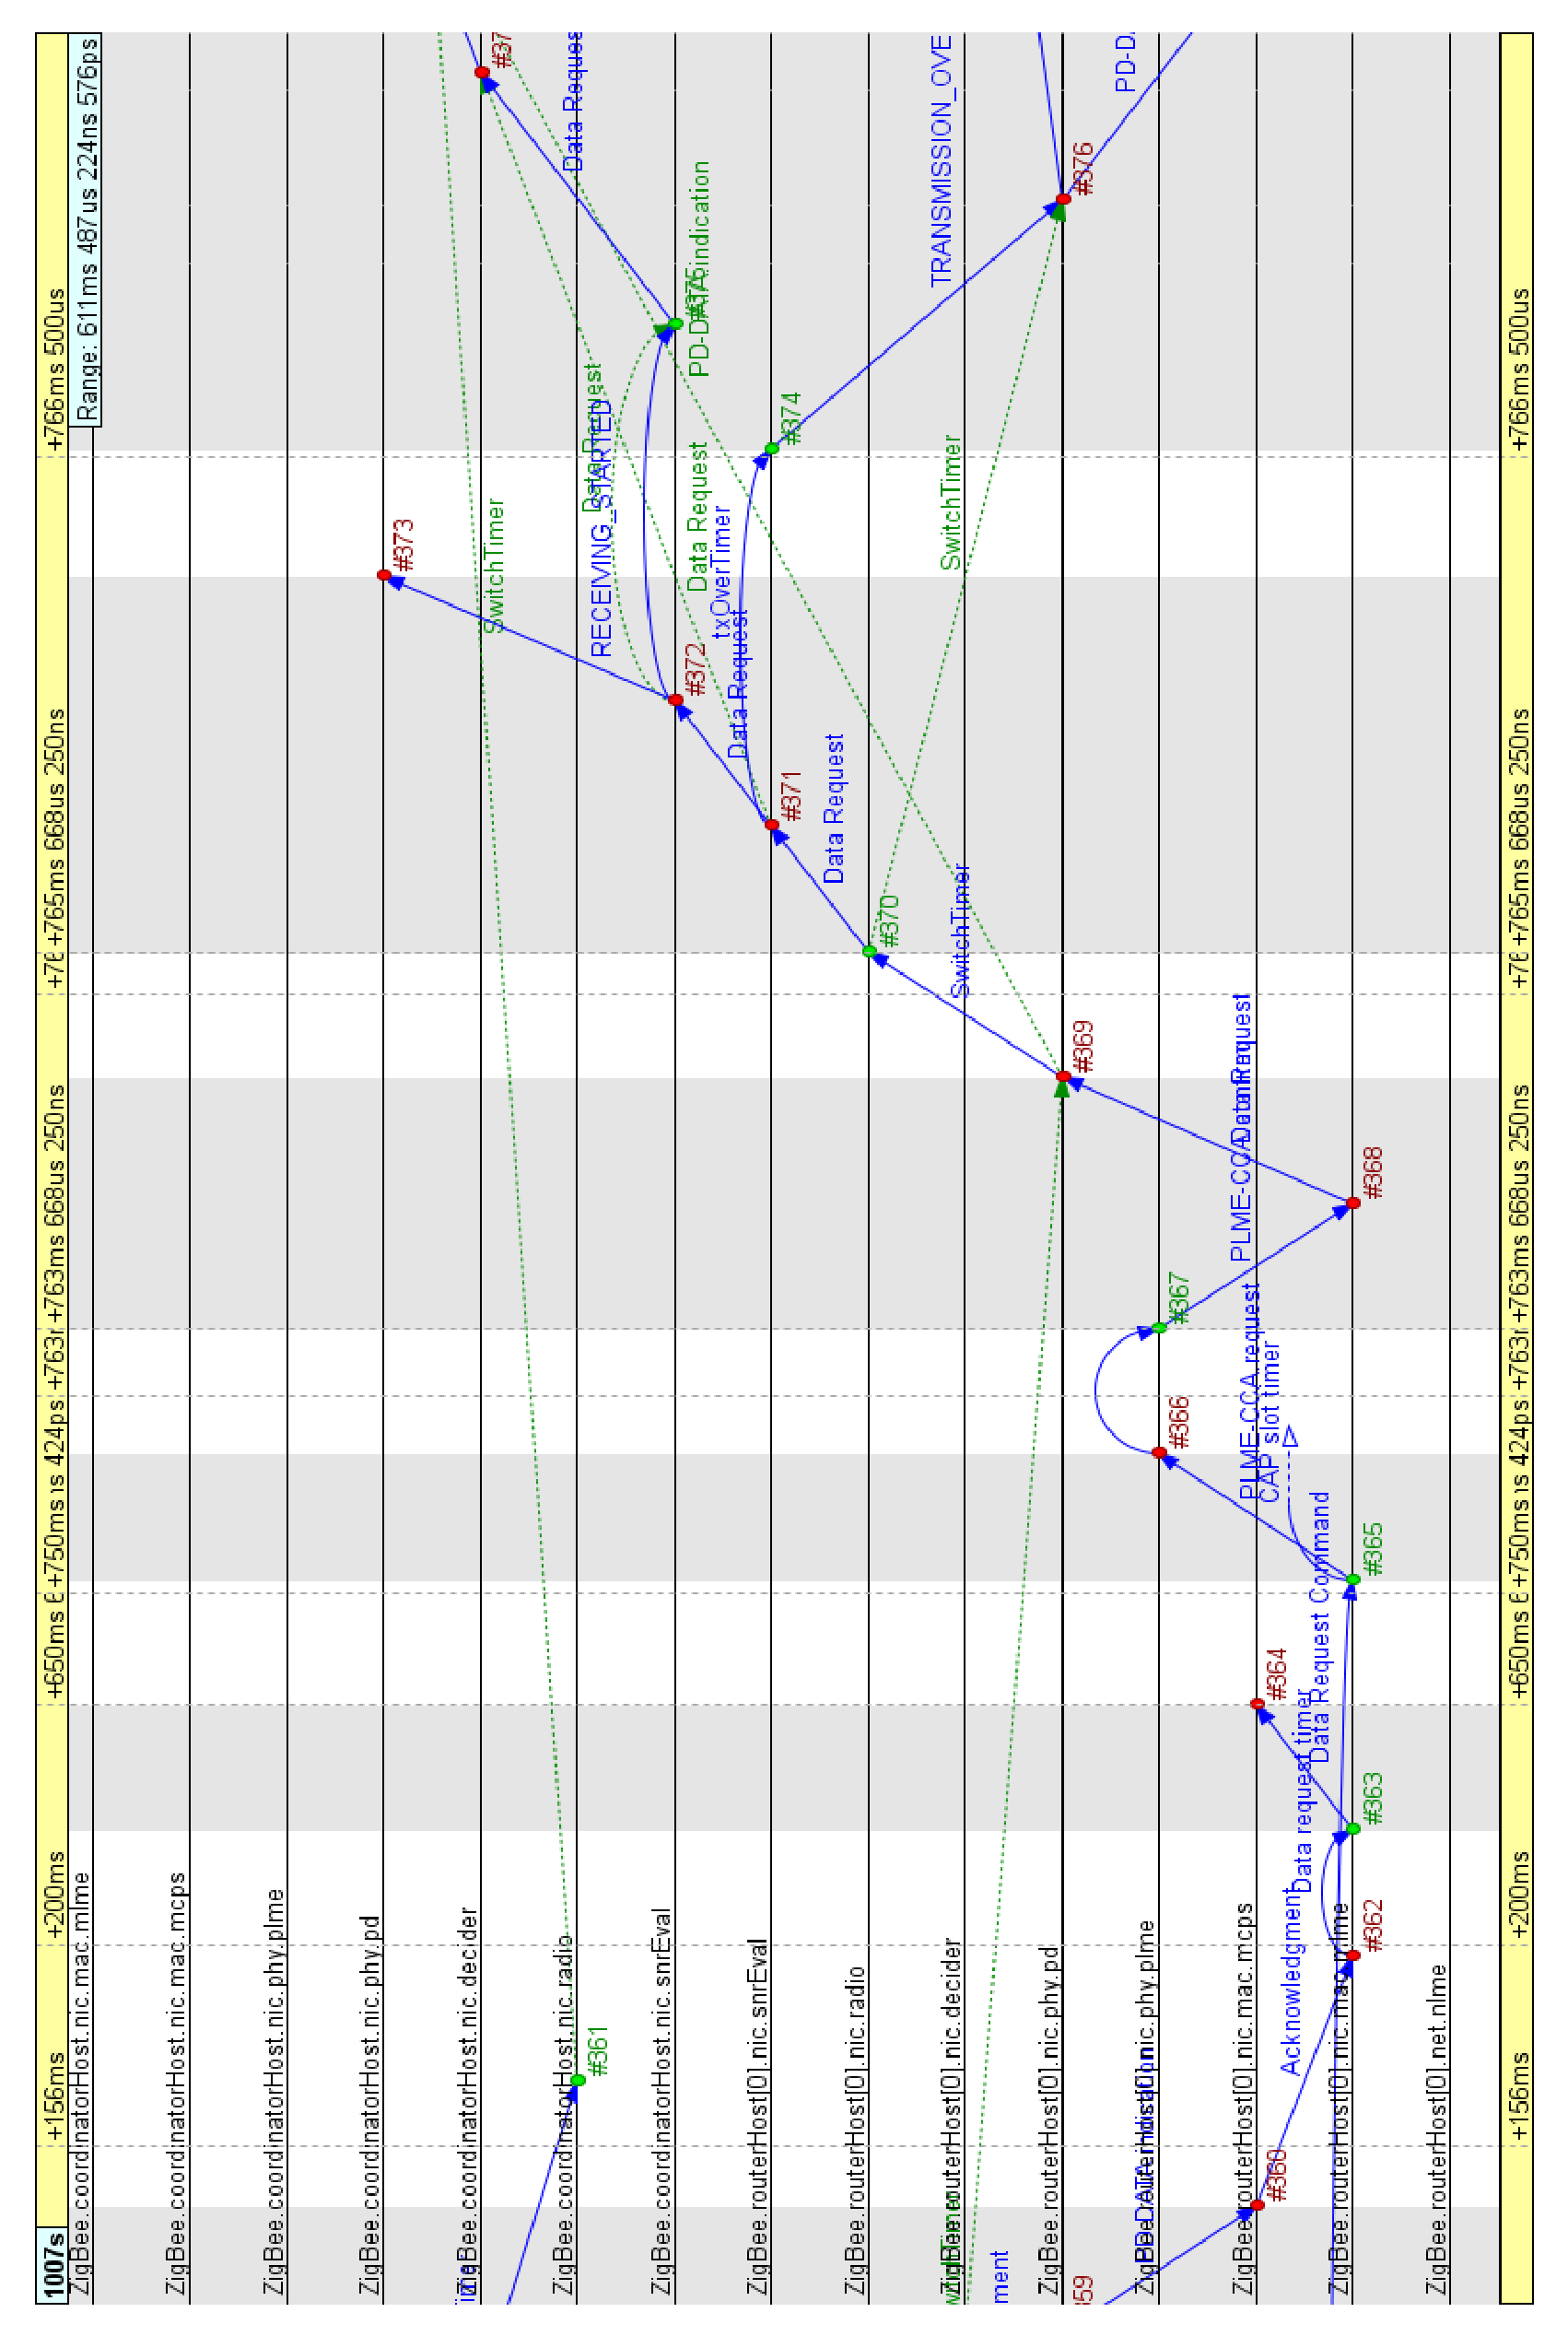
\includegraphics[width=140mm]{figures/chart_data_request}
\caption{Žiadosť o zaslanie dát, CCA procedúra}
\label{fig:chart_data_request}
\end{center}
\end{figure}

\begin{figure}[htbp]
\begin{center}
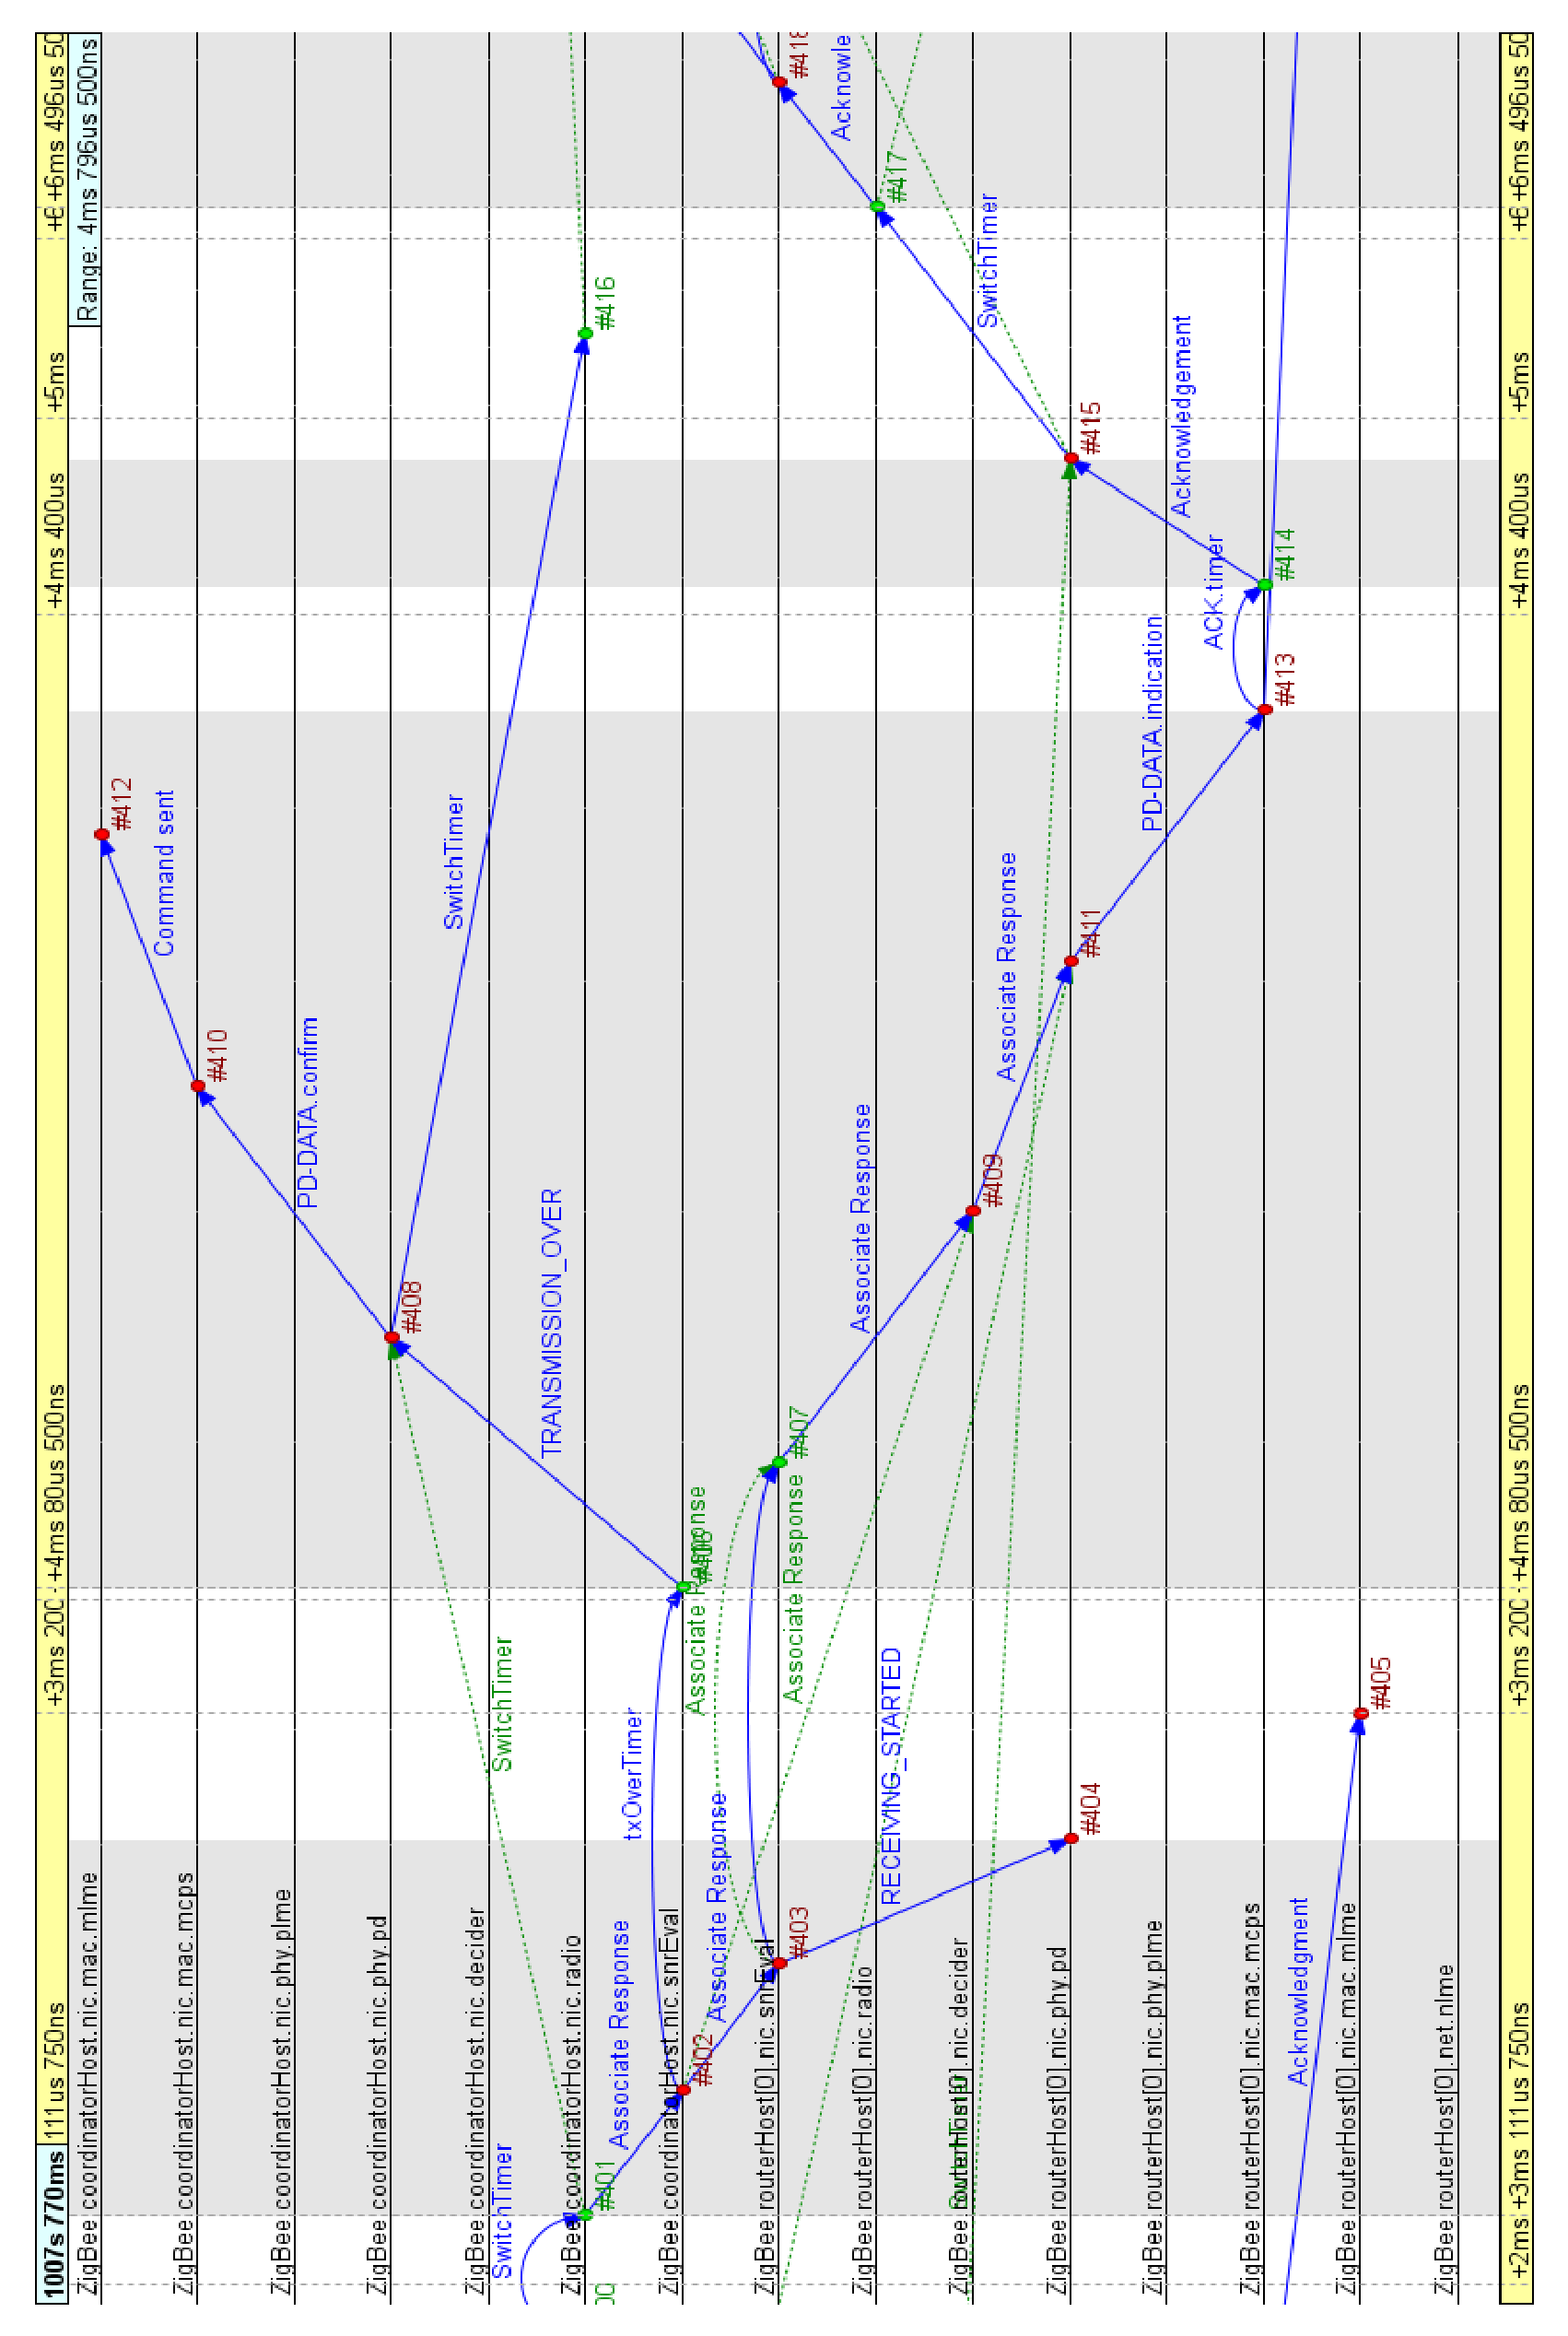
\includegraphics[width=140mm]{figures/chart_associate_response}
\caption{Odpoveď na žiadosť o asociáciu, jej spracovanie}
\label{fig:chart_associate_response}
\end{center}
\end{figure}